\documentclass{wptemp}
\usepackage{adjustbox}
\usepackage{setspace}\doublespacing%\onehalfspacing
\usepackage{natbib}
\newcommand{\GG}[1]{}
\usepackage{booktabs}
\usepackage{siunitx}
\newcolumntype{d}{S[input-symbols = ()]}\singlespacing
\doublespacing
\usepackage{lscape}
\newcommand{\ts}{\textsuperscript}
\usepackage{threeparttable}
\usepackage{threeparttablex}

% *****************************************************************
% Estout LaTeX wrapper
% *****************************************************************

%%Original code developed by Jörg Weber: see
%% https://www.jwe.cc/2012/03/stata-latex-tables-estout/
%% and
%% https://www.jwe.cc/blog/



\let\estinput=\input % define a new input command so that we can still flatten the document

\newcommand{\estwide}[3]{
		\vspace{.75ex}{
			%\textsymbols% Note the added command here
			\begin{tabular*}
			{\textwidth}{@{\hskip\tabcolsep\extracolsep\fill}l*{#2}{#3}}
			\toprule
			\estinput{#1}
			\bottomrule
			\addlinespace[.75ex]
			\end{tabular*}
			}
		}	

\newcommand{\estauto}[3]{
		\vspace{.75ex}{
			%\textsymbols% Note the added command here
			\begin{tabular}{l*{#2}{#3}}
			\toprule
			\estinput{#1}
			\bottomrule
			\addlinespace[.75ex]
			\end{tabular}
			}
		}

% Allow line breaks with \ in specialcells
\newcommand{\specialcell}[2][c]{%
    \begin{tabular}[#1]{@{}c@{}}#2\end{tabular}
}

\newcommand{\sym}[1]{\rlap{#1}}% Thanks David Carlisle


%%%%%%%%%%% End of wrapper %%%%%%%%%%%%%%%%%%%%%
    
%%%%%%%%%%% TiKz %%%%%%%%%%%%%%%%%%%%%
\usepackage{tikz}
\usetikzlibrary{shapes.geometric, arrows}

\tikzstyle{startstop} = [rectangle, rounded corners, minimum width=3cm, minimum height=1cm,text centered, draw=black, fill=red!30]

\tikzstyle{io} = [trapezium, trapezium left angle=70, trapezium right angle=110, minimum width=3cm, minimum height=1cm, text centered, text width =5cm, draw=black, fill=blue!30]

\tikzstyle{process} = [rectangle, minimum width=3cm, minimum height=1cm, text centered, text width =5cm, draw=black, fill=orange!30]

\tikzstyle{decision} = [diamond, minimum width=3cm, minimum height=1cm, text centered, draw=black, fill=green!30]

\tikzstyle{arrow} = [thick,->,>=stealth]

\begin{document}

\linespread{1}{\title{{\fontfamily{ptm}\selectfont{\Large{\MakeUppercase{Democracy and Ethnic Favoritism: Evidence \\
from Africa}}}}\thanks{I am so grateful to Willa Friedman for her advice, comments and support. I thank Nathan Canen, Aimee Chin, German Cubas, Chinhui Juhn, Vikram Maheshri and the participants of the Empirical Microeconomics Workshop at the University of Houston for their comments and feedback. Abhi Basvoju provided excellent research assistance.}
}
}
	\author{{\fontfamily{pbk}\selectfont\large{\textsc{Hussain Hadah}}\thanks{Department of Economics, University of Houston, Science Building 3581 Cullen Boulevard Suite 230, Houston, TX 77204-5019, United States (e-mail: \email{hhadah@uh.edu}).}}}
	\date{\fontfamily{pbk}\selectfont\normalsize{\textsc{\today}}}
	\maketitle

\begin{center}
\href{https://hussainhadah.com/workingpaper/ethnicfav/HussainHadahEthFav.pdf}{\textcolor{green!15!black!30!blue}{\footnotesize{\textsc{Click Here to Get the Most Updated Version}}}}
\end{center}

\begin{abstract} 
What is the effect of democracy on ethnic favoritism? I estimate the relationship between co-ethnicity and five outcomes of public good provision – education, infant health, wealth, access to clean drinking water and access to electricity – using data from twenty-one African countries. Following previous research, I use variation in co-ethnicity across ethnic groups and over time. I first estimate the relationship between these five outcomes and co-ethnicity in the full sample and then split the analysis between anocracies and democracies. I find mixed evidence of ethnic favoritism in the full sample. I find more evidence of co-ethnic targeting when comparing within democracies only and within anocracies only.

\keywords{Ethnic favoritism; democracy; dictatorships; institutions.}
\JEL{D3, O1, O2.}
\end{abstract}

\thispagestyle{empty}
\clearpage
\pagenumbering{arabic}


\begin{table}

\caption{Summary Statistics \label{tabsum}}
\centering
\begin{threeparttable}
\resizebox{\linewidth}{!}{
\begin{tabular}[t]{lc}
\toprule
\textbf{Characteristic} & \textbf{N = 1,387,301}\\
\midrule
Age & \makecell[c]{29 \\(10) \\[10, 98]}\\
Total children ever born & \makecell[c]{3.02 \\(3.99) \\[0.00, 99.00]}\\
Total number of household members & \makecell[c]{7.3 \\(5.0) \\[1.0, 80.0]}\\
Has electricity & 0.31\\
Currently working & 0.55\\
Wealth Quintile & \\
\hspace{1em}1 & 0.19\\
\hspace{1em}2 & 0.18\\
\hspace{1em}3 & 0.19\\
\hspace{1em}4 & 0.20\\
\hspace{1em}5 & 0.24\\
Total years of education & \makecell[c]{5.0 \\(4.7) \\[0.0, 26.0]}\\
Completed primary school & 0.65\\
Urban & 0.36\\
Literacy & 0.58\\
\bottomrule
\multicolumn{2}{l}{\rule{0pt}{1em}\textsuperscript{1} Mean\ \  (SD)\ \  [Range]; \%}\\
\end{tabular}}
\begin{tablenotes}
\item[1] Data source is the Demographic and Health Surveys (DHS).
\end{tablenotes}
\end{threeparttable}
\end{table}



\begin{figure}[!htb]
\centering
\caption{Democracy in sample countries from 1980 to 2000.}
\label{fig1}
\begin{subfigure}{.48\textwidth}
\centering
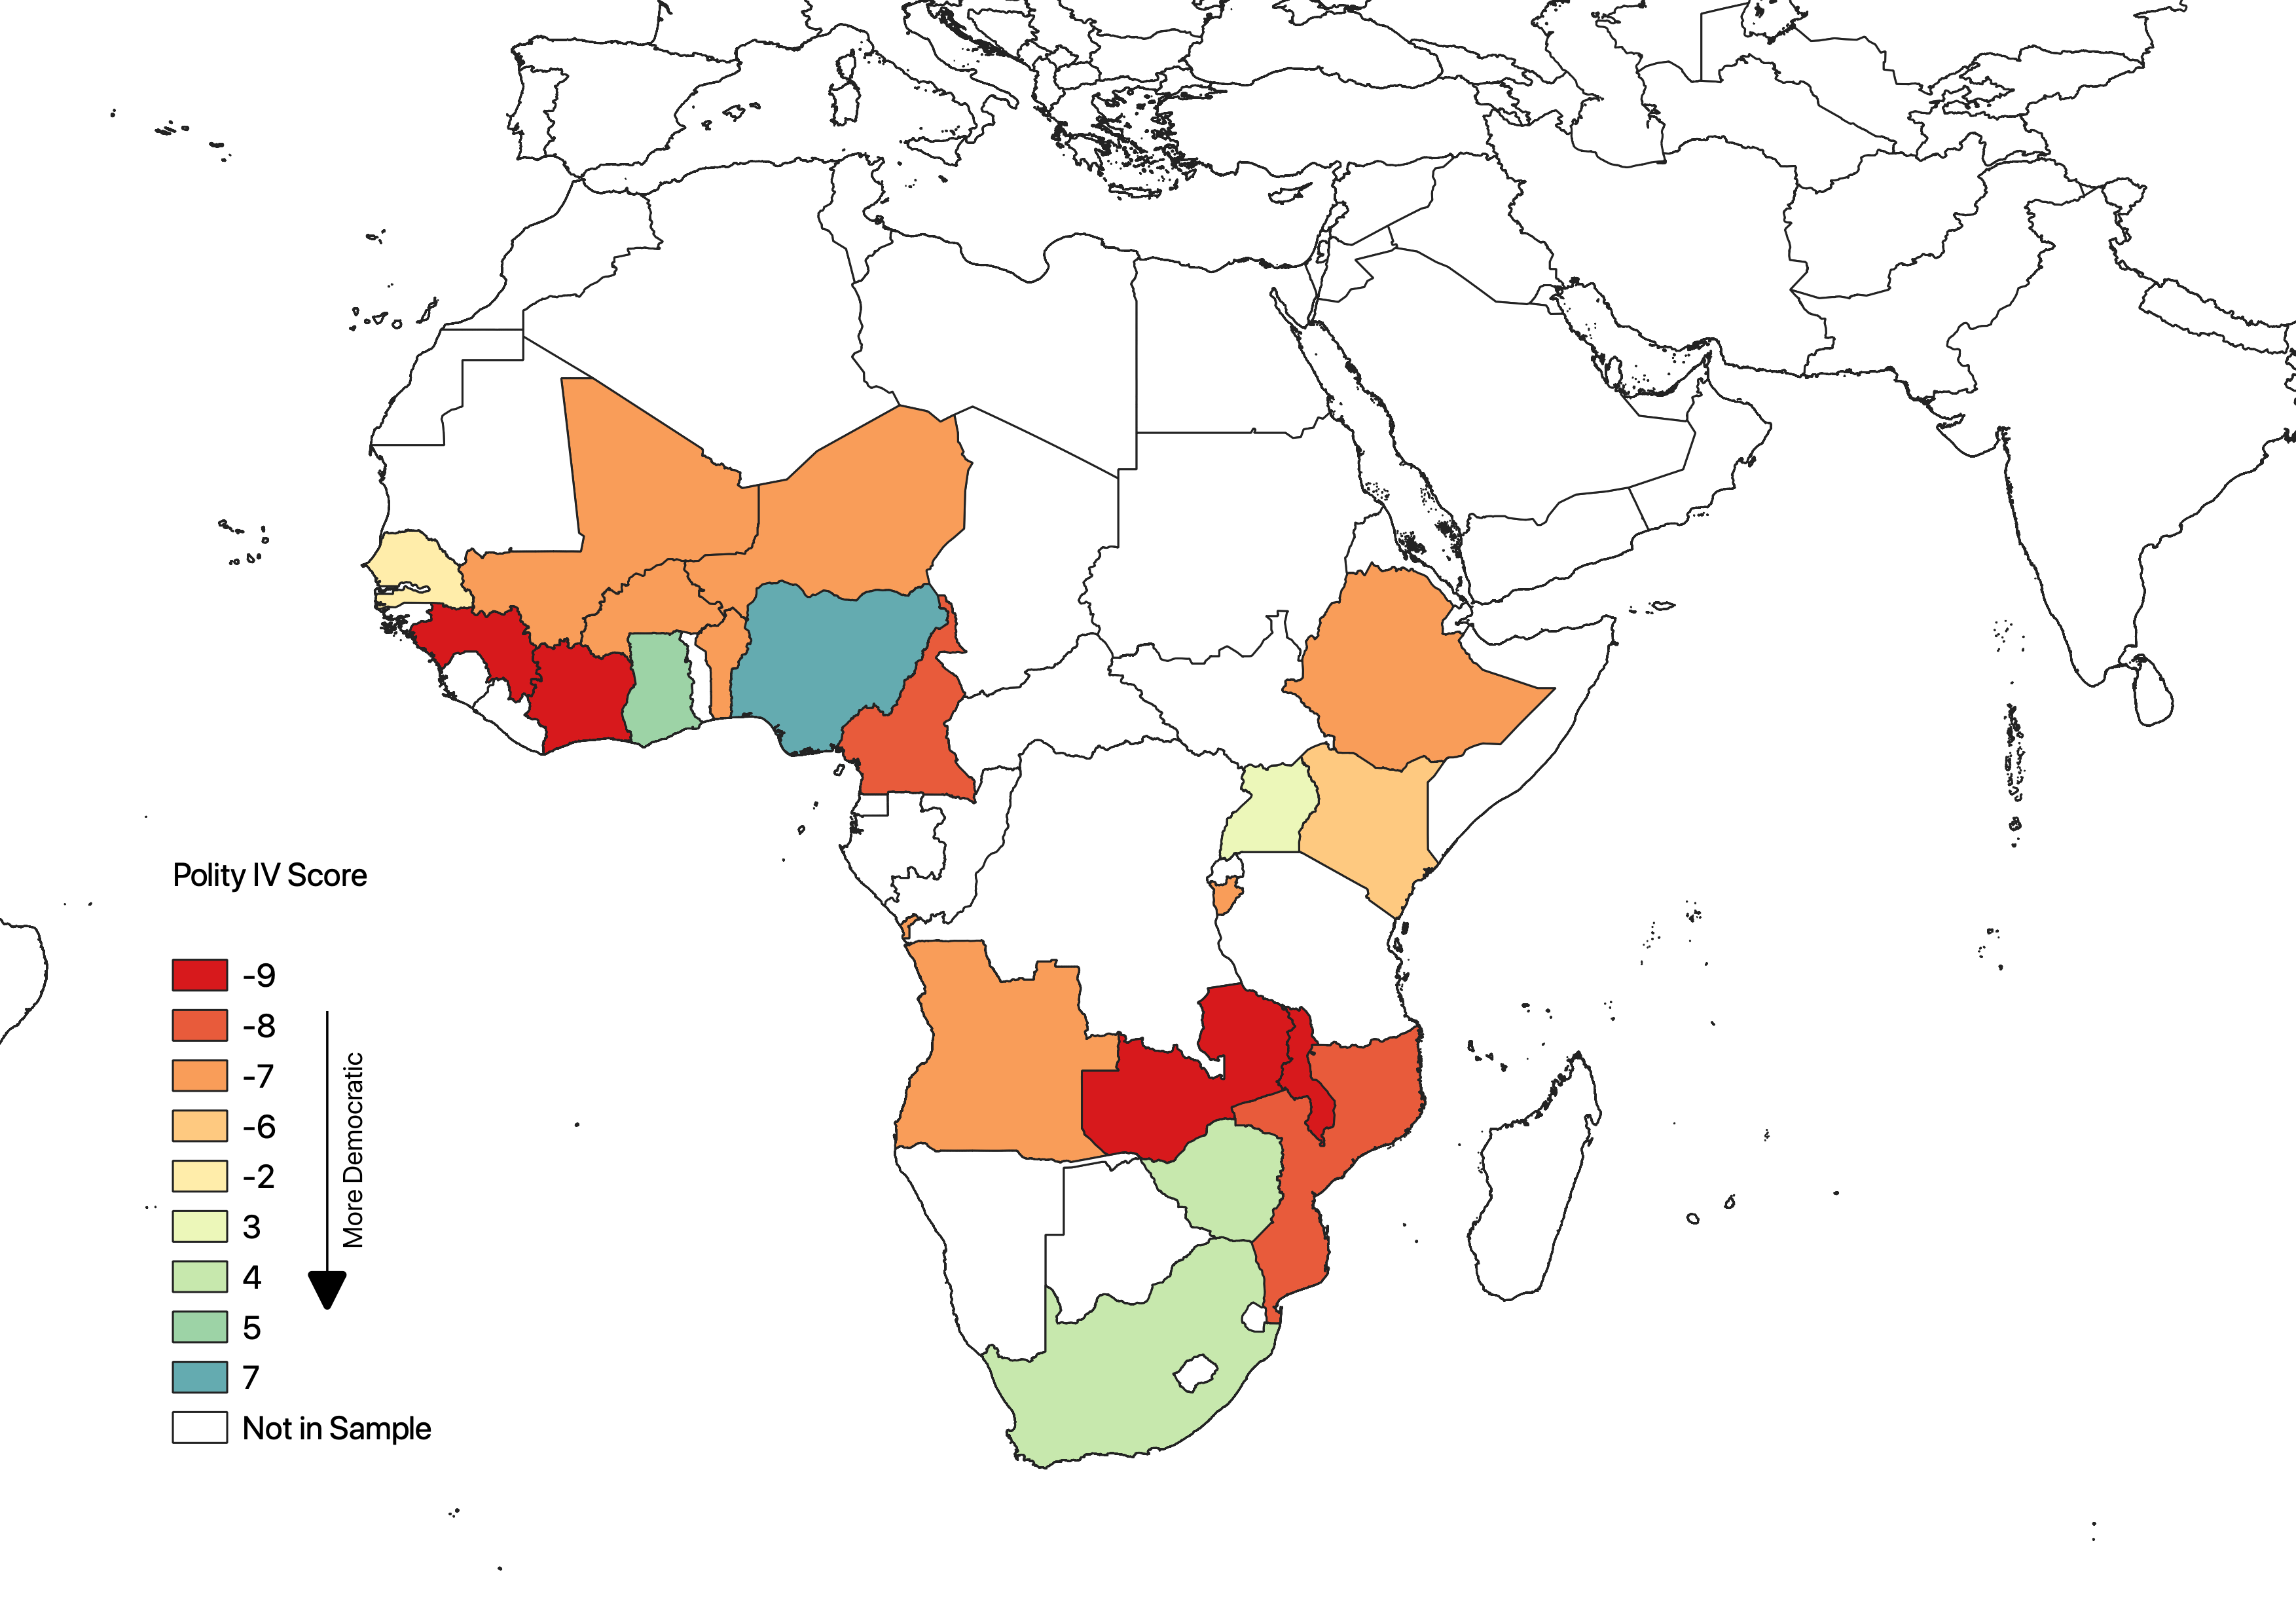
\includegraphics[width=.9\linewidth]{1980.png}
\caption{Polity Scores in 1980.}
\label{fig1980}
\end{subfigure}
\centering
%Second graph
\begin{subfigure}{.48\textwidth}
\centering
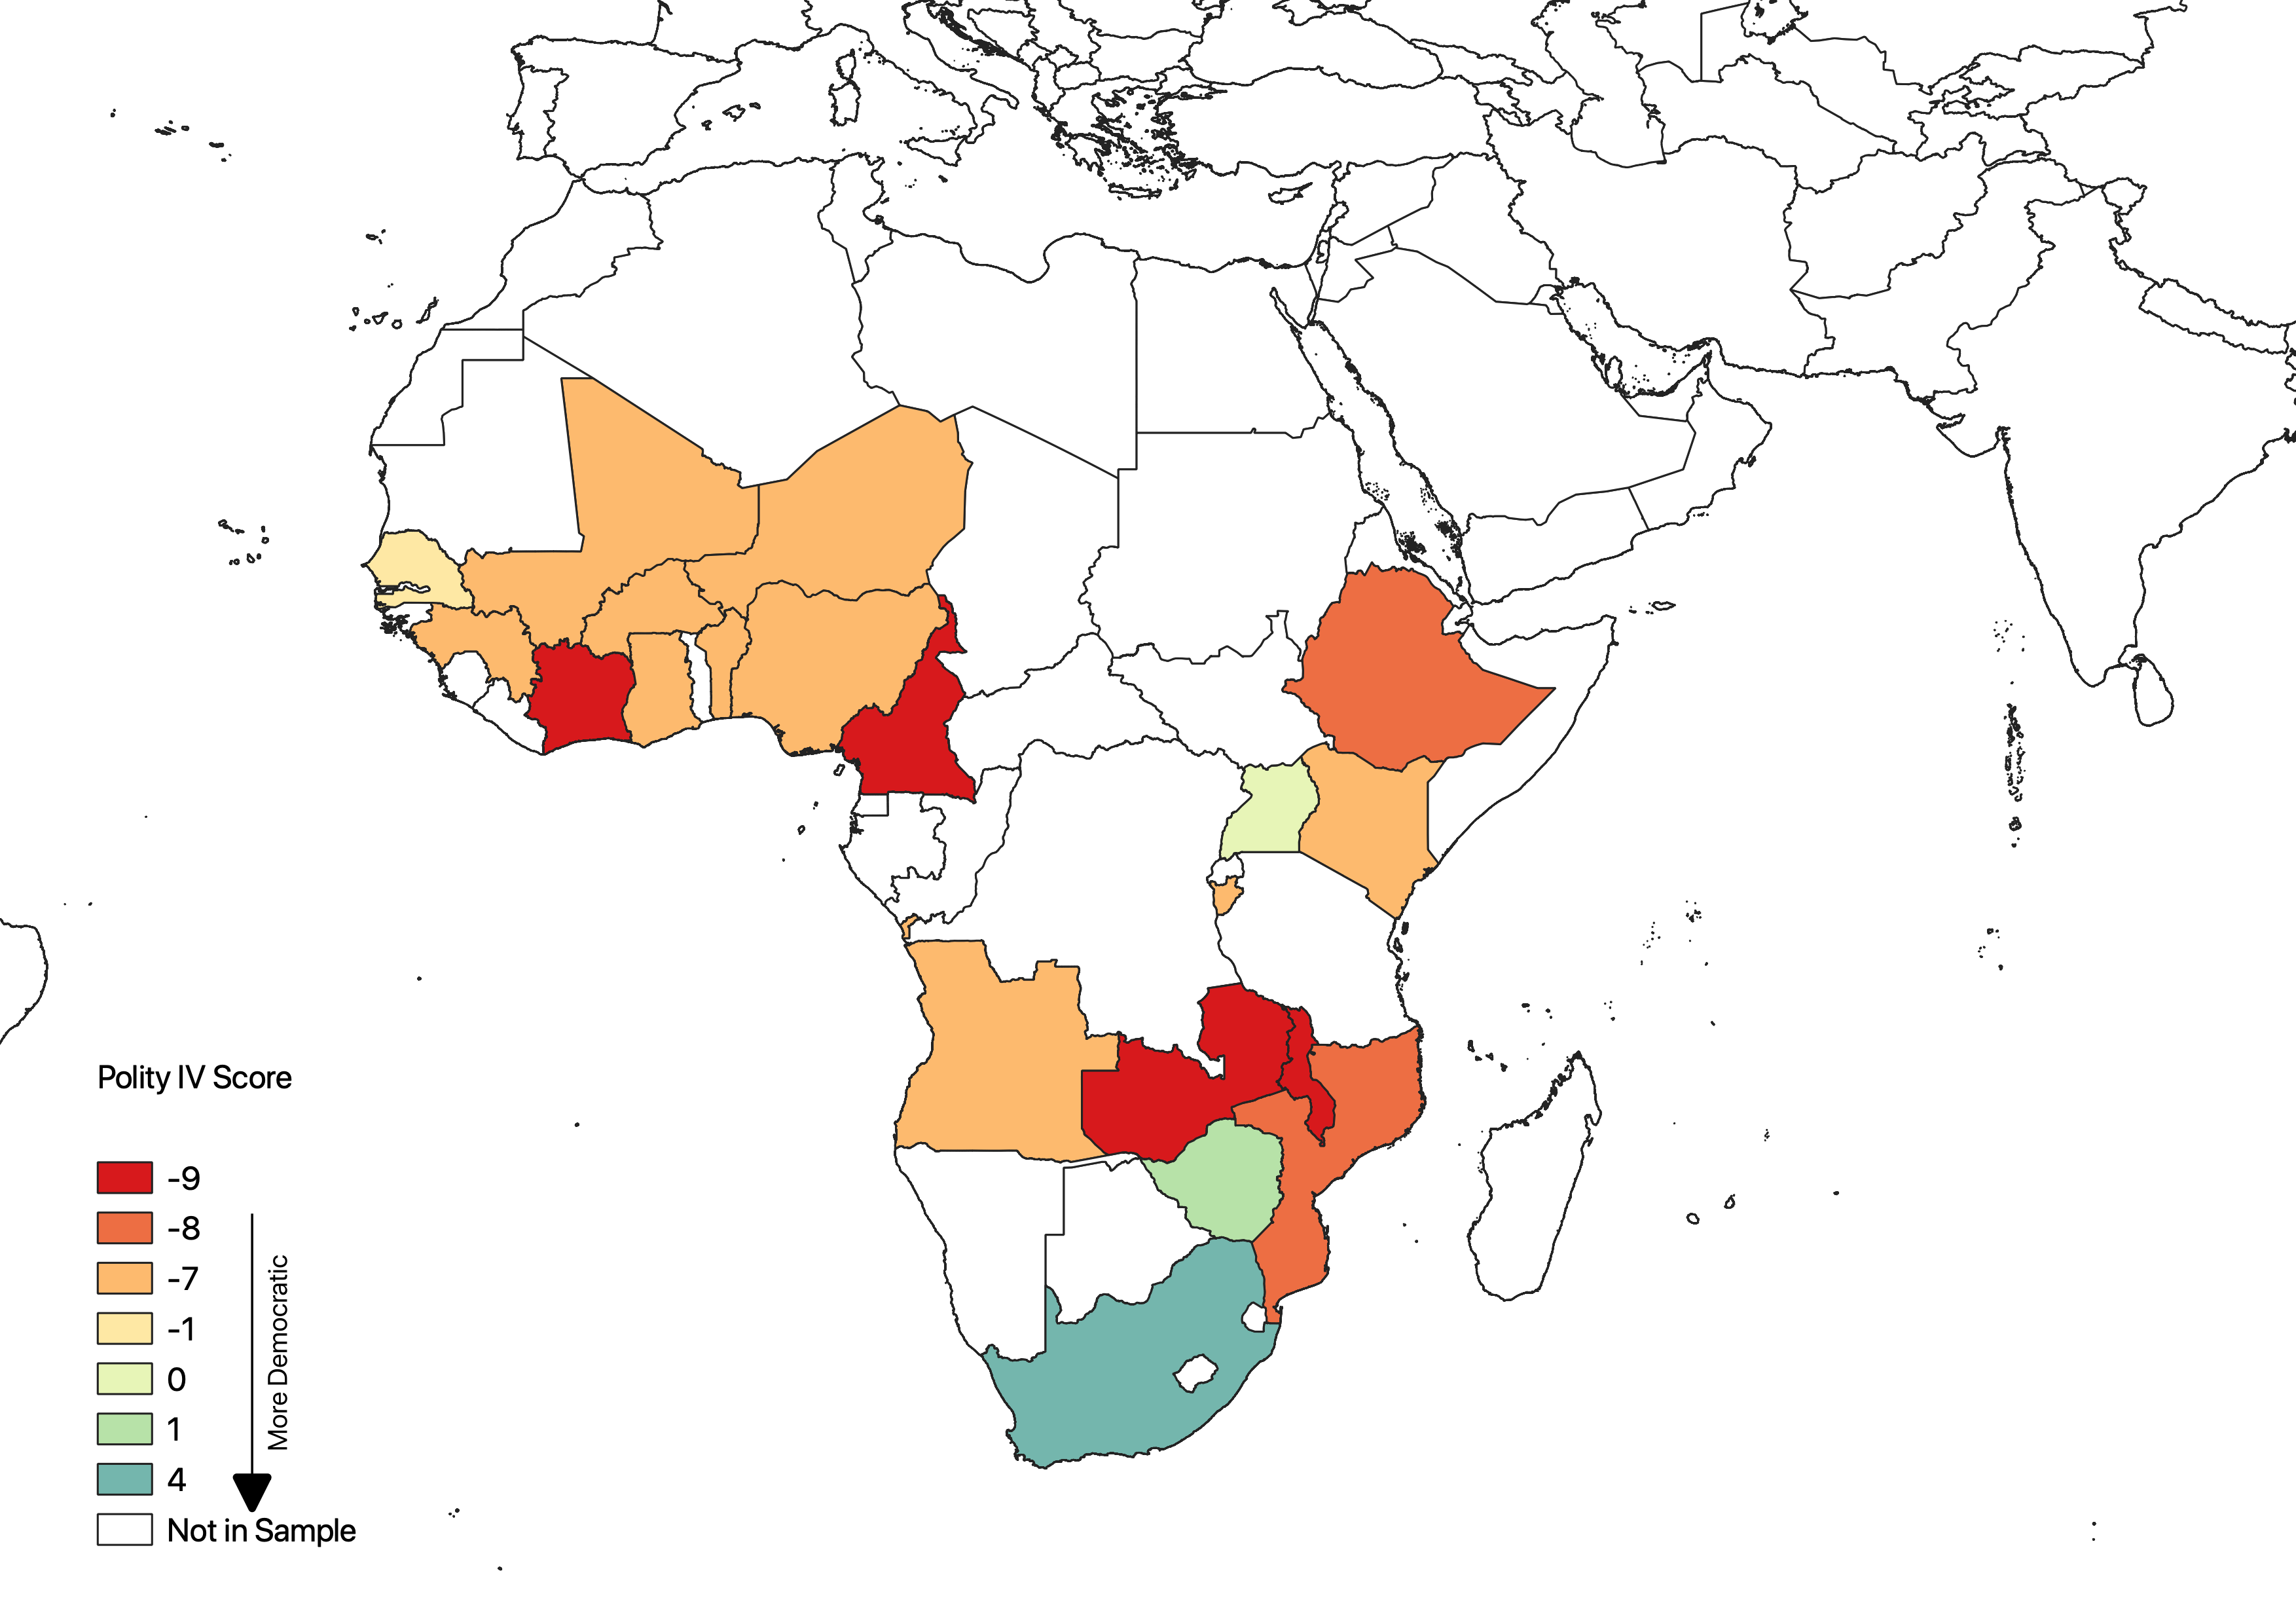
\includegraphics[width=.9\linewidth]{1985.png}
\caption{Polity Scores in 1985.}
\label{fig1985}
\end{subfigure}
%Third
\begin{subfigure}{.48\textwidth}
\centering
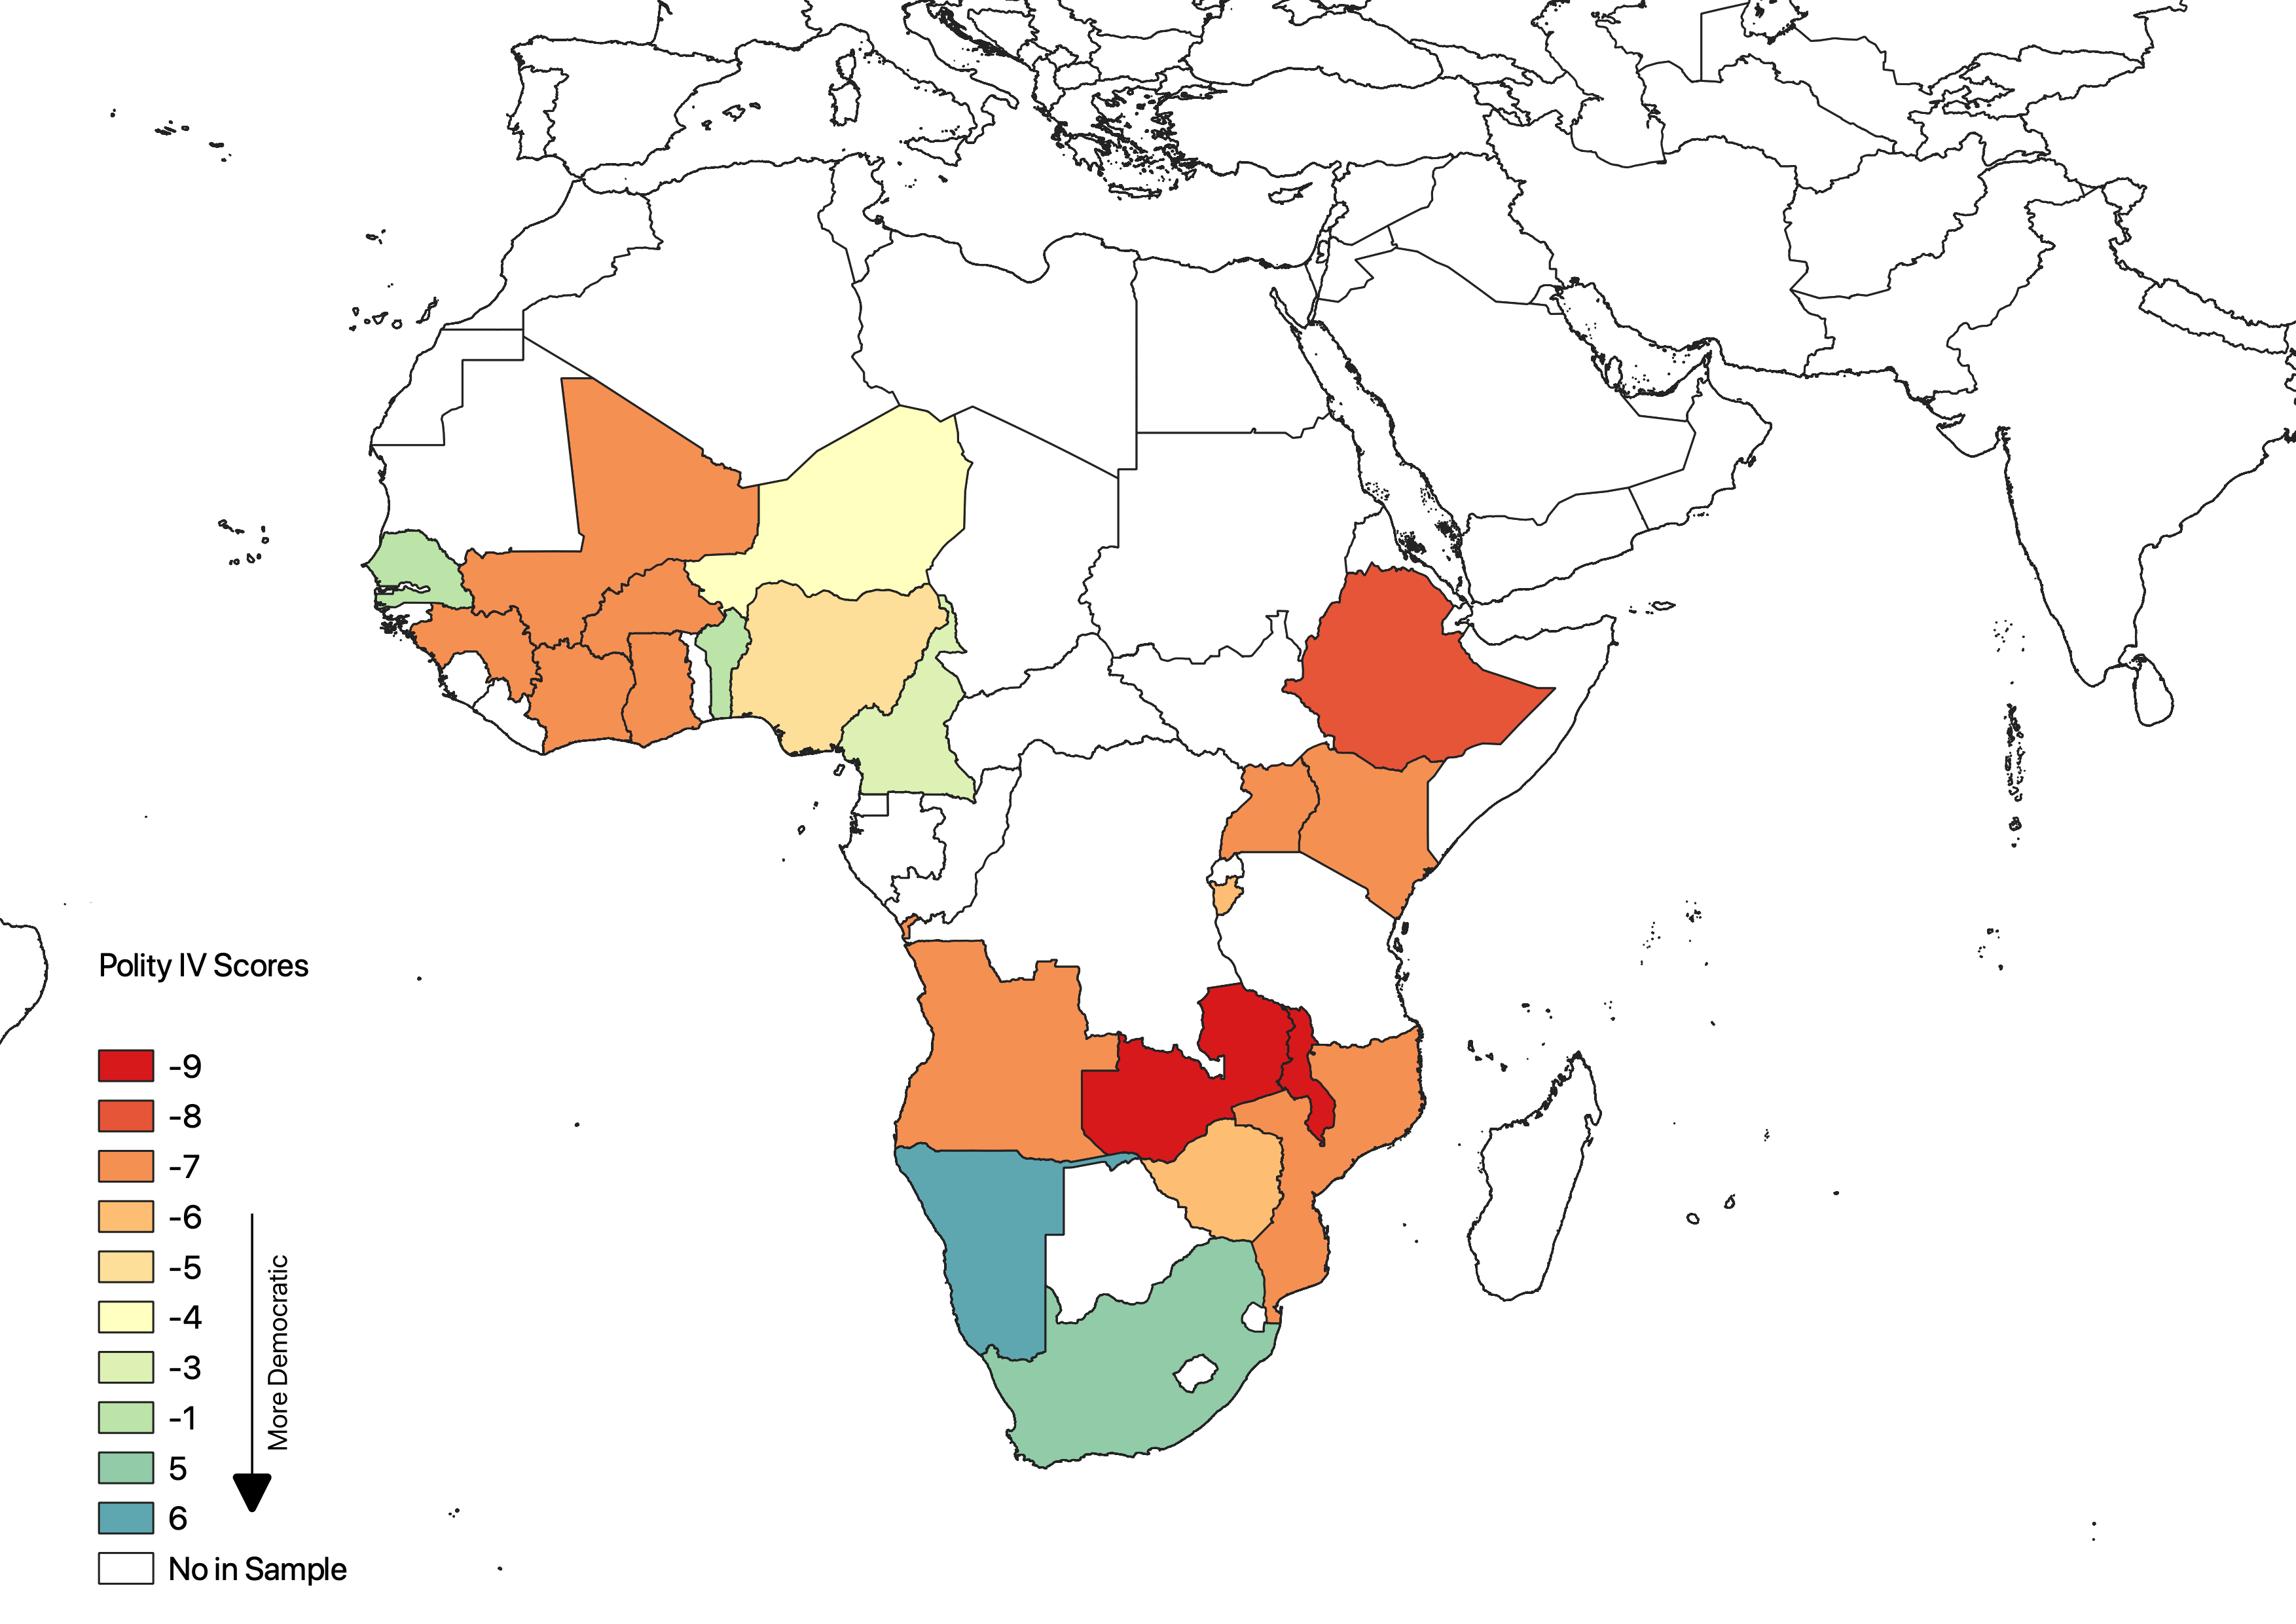
\includegraphics[width=.9\linewidth]{1990.png}
\caption{Polity Scores in 1990.}
\label{fig1990}
\end{subfigure}
% Fourth
\begin{subfigure}{.48\textwidth}
\centering
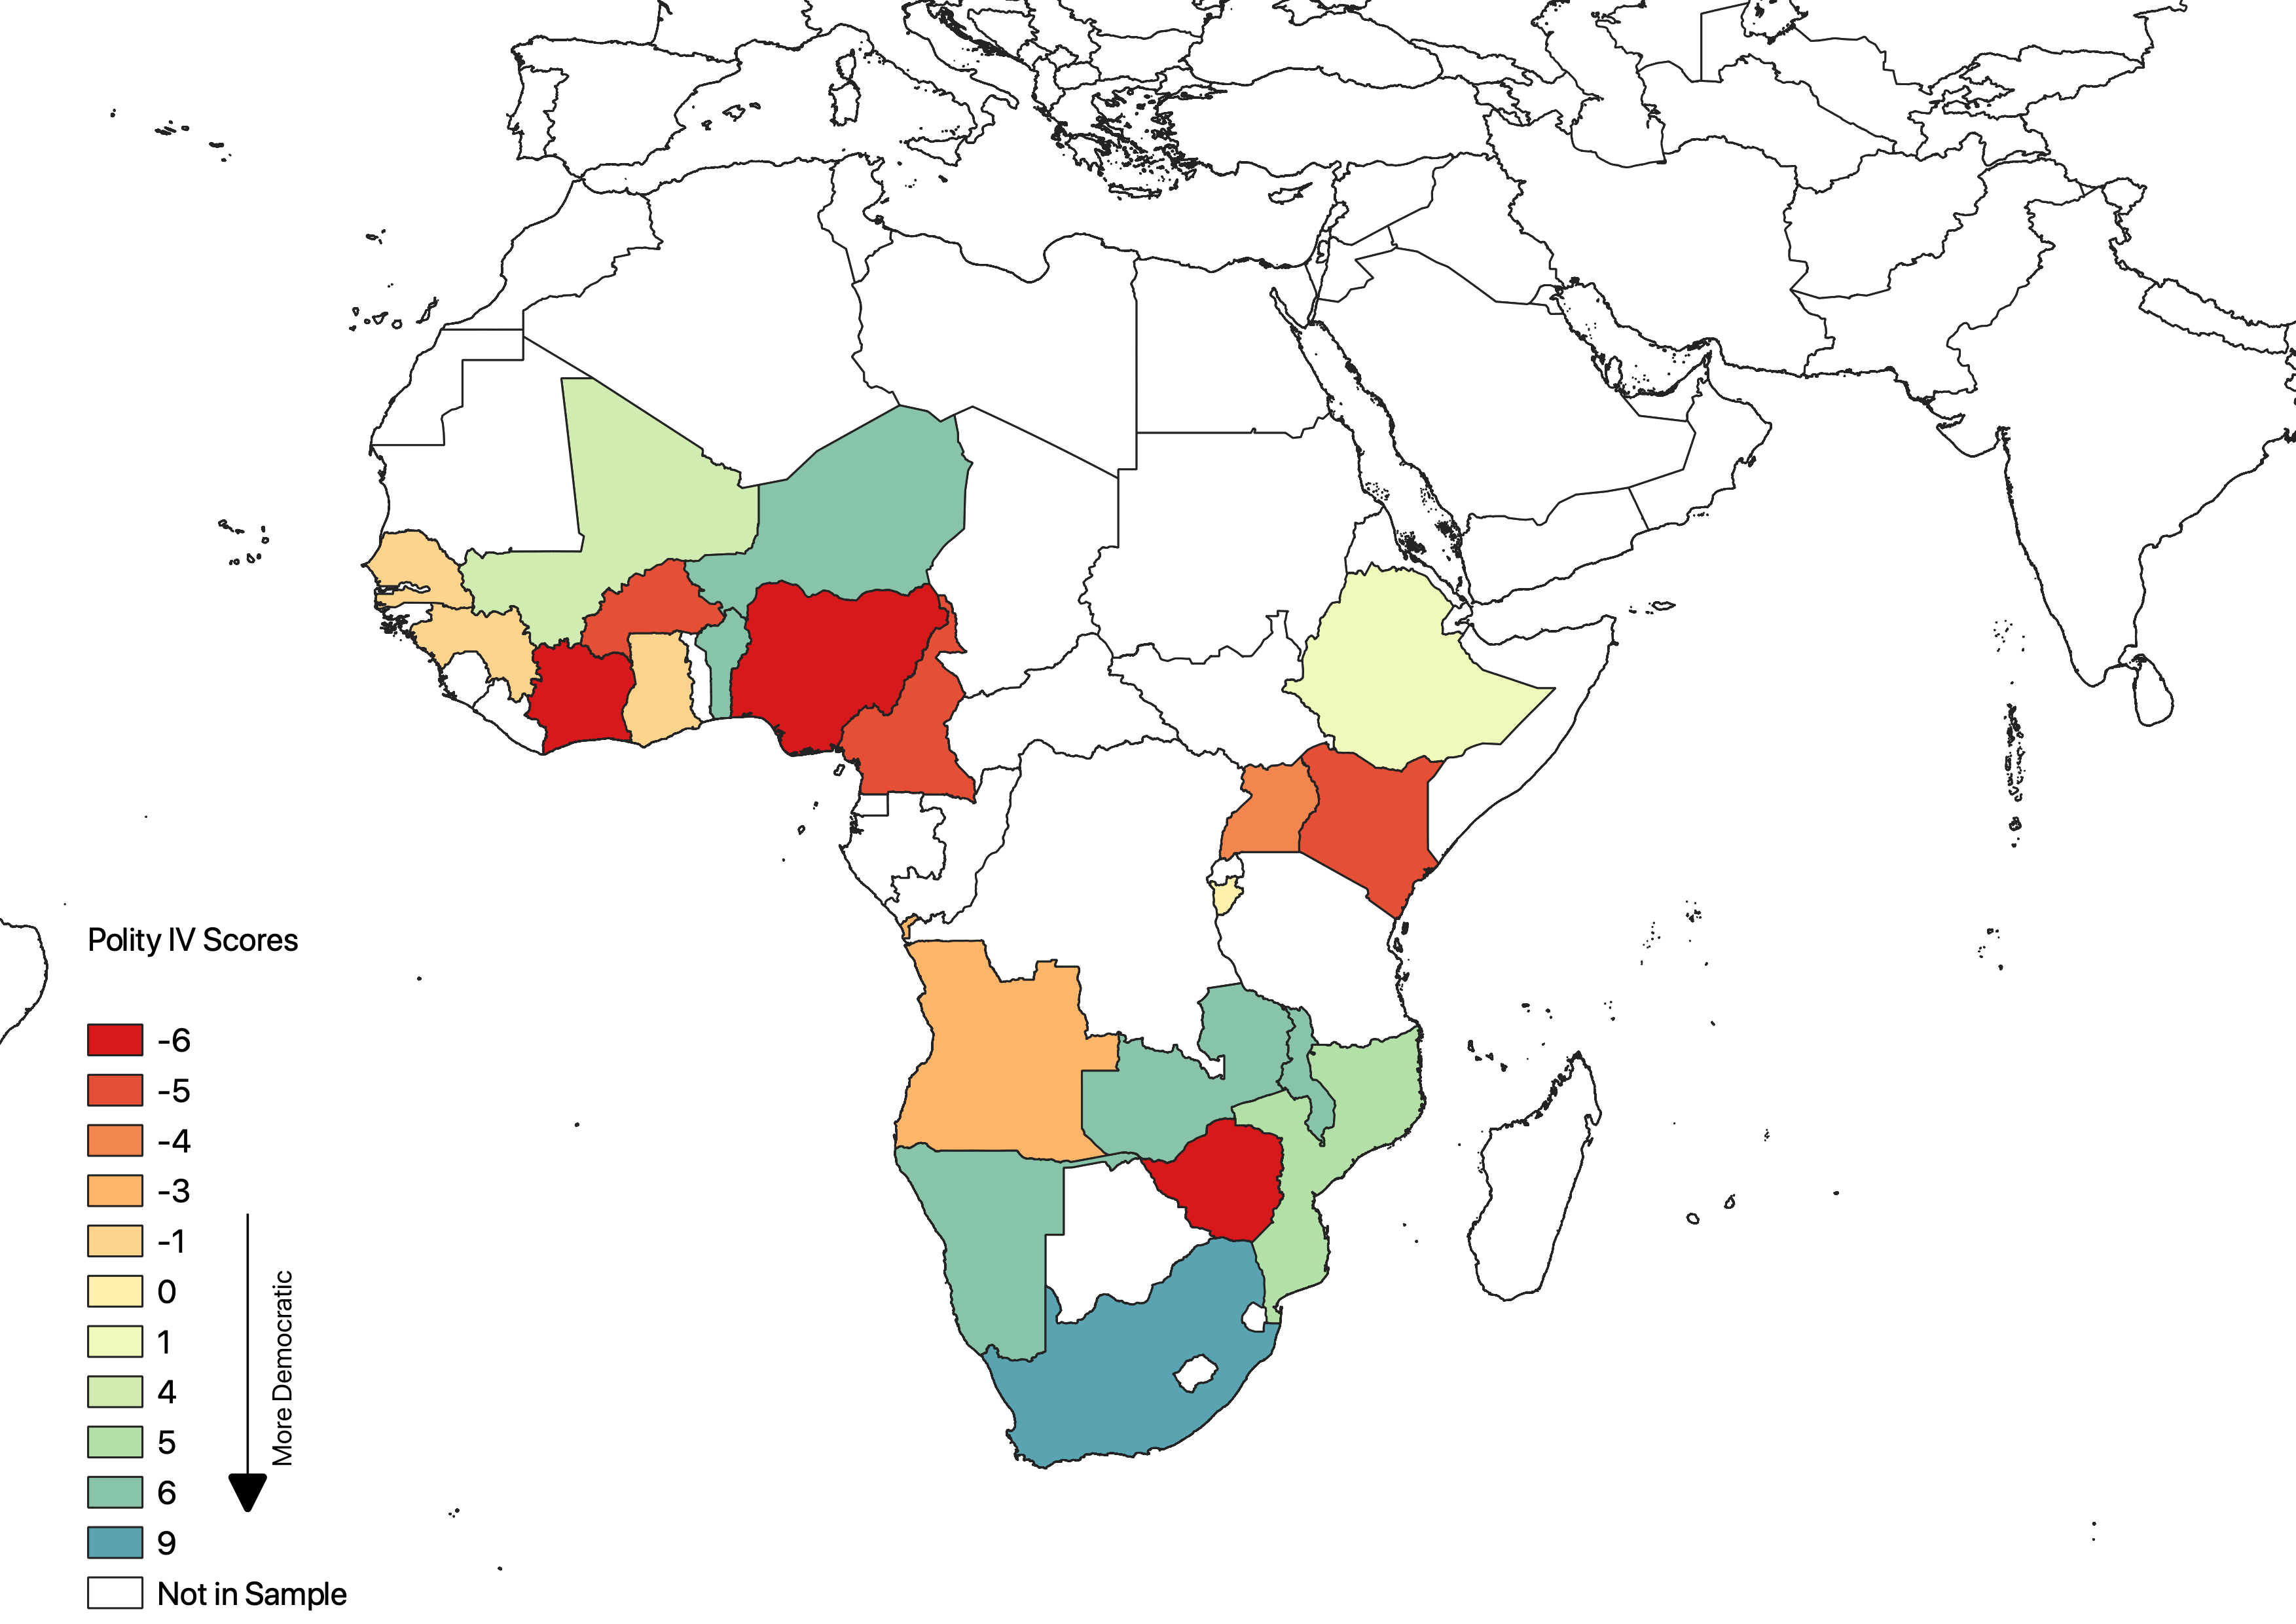
\includegraphics[width=.9\linewidth]{1995.png}
\caption{Polity Scores in 1995.}
\label{fig1995}
\end{subfigure}
%Fifth
\begin{subfigure}{.9\textwidth}
\centering
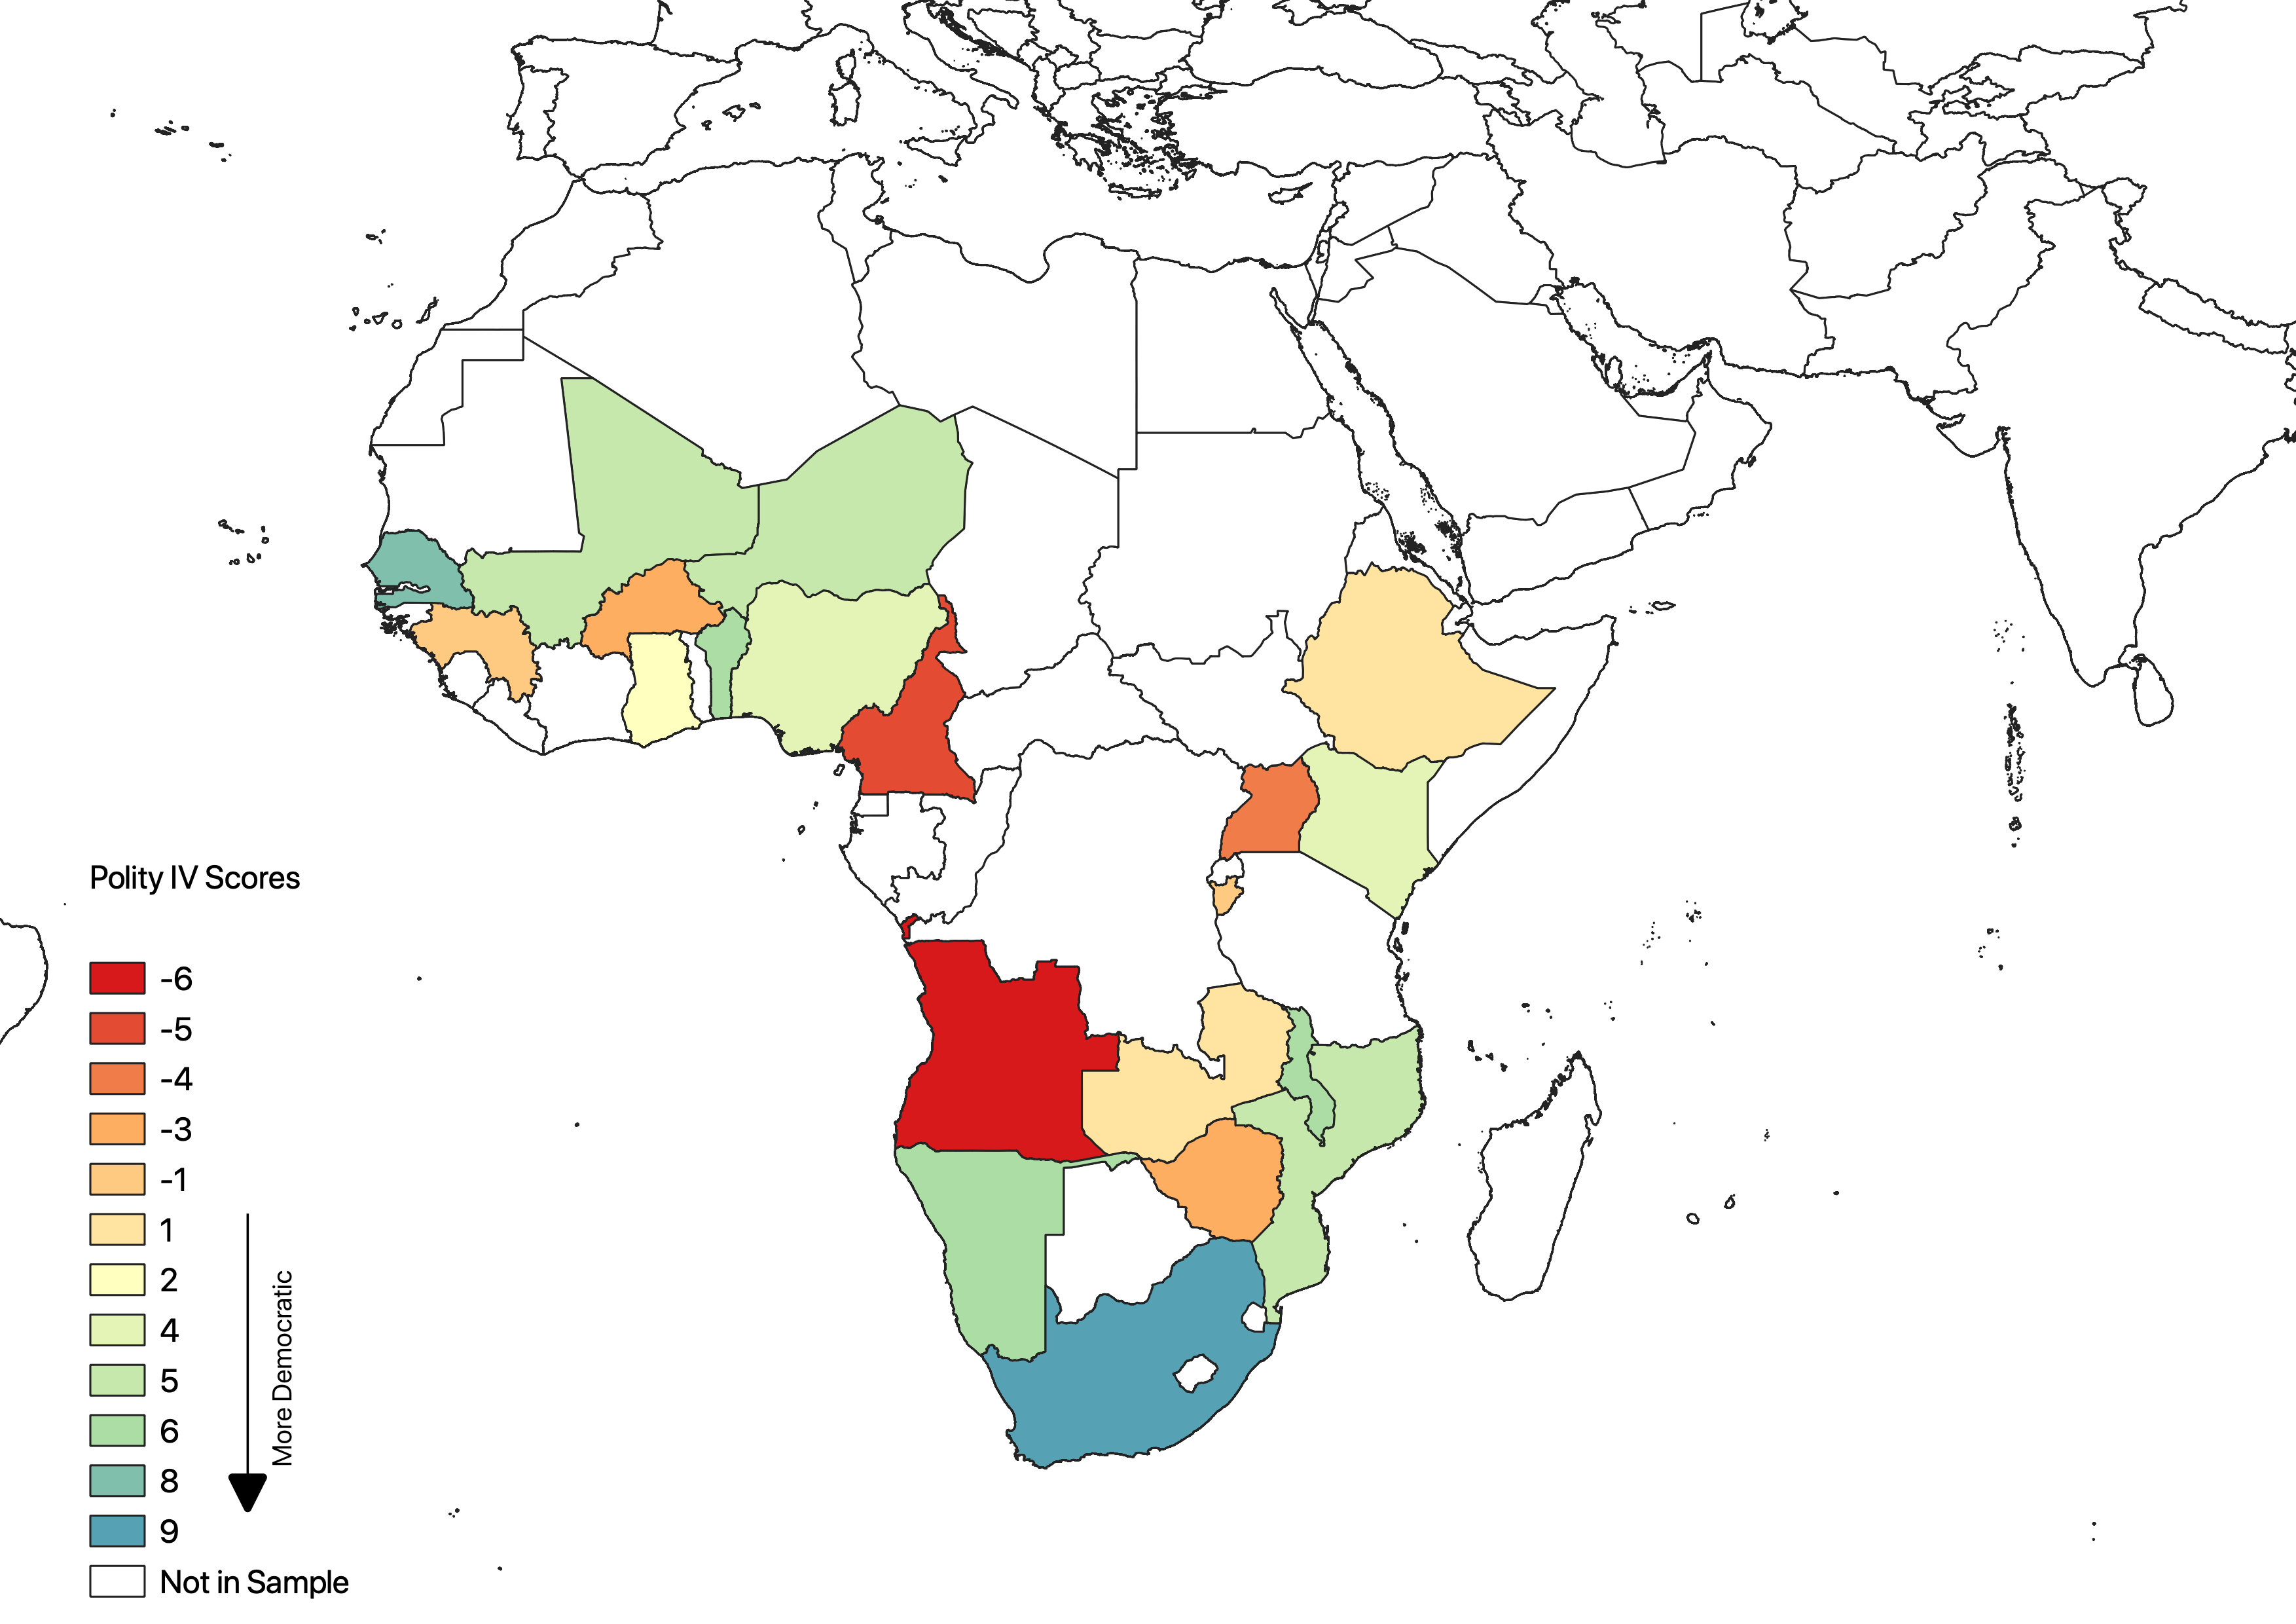
\includegraphics[width=.5\linewidth]{2000.png}
\caption{Polity Scores in 2000}
\label{fig2000}
\end{subfigure}

\note{In this figure, I present the changes in Polity IV scores in the countries I am studying from 1980 to 2000. Notice Africa's democratization.}

\end{figure}



\begin{table}[!h]

\caption{Ethnic favoritism results \label{tab:eth}}
\centering
\resizebox{\linewidth}{!}{
\begin{threeparttable}
\begin{tabular}[t]{lccccc}
\toprule
  & \specialcell{(1) \\ Schooling} & \specialcell{(2) \\ Infant Survival} & \specialcell{(3) \\ Wealth} & \specialcell{(4) \\ Electrification} & \specialcell{(5) \\ Clean Water}\\
\midrule
Coethnic & \num{-0.038} & \num{0.005} & \num{0.001} & \num{0.042}*** & \num{-0.028}\\
 & (\num{0.024}) & (\num{0.004}) & (\num{0.023}) & (\num{0.016}) & (\num{0.032})\\
\midrule
Mean & \num{0.649} & \num{0.905} & \num{0.275} & \num{0.351} & \num{0.216}\\
N & \num{1146305} & \num{2516753} & \num{756737} & \num{822353} & \num{822353}\\
\bottomrule
\multicolumn{6}{l}{\rule{0pt}{1em}* p $<$ 0.1, ** p $<$ 0.05, *** p $<$ 0.01}\\
\end{tabular}
\begin{tablenotes}
\item[1] \footnotesize{In this table, I am reporting the estimates of equation \ref{eqFR1}. 
                      I present the results of the effect of ethnic favoritism on primary school completions 
                      in column 1, infant survival in column 2, top wealth quintile in column 3, electrification in 
                      column 4 and access to clean drinking water in column 4. Primary school completion is a 
                      dummy variable that is equal to one if a person completed primary school and zero otherwise. 
                      Infant survival is a dummy variable that is equal to one if an infant survived the first 12 
                      months of life. Wealth is a dummy variable that is equal to one if a person belongs to the top 
                      wealth quintile. Electrification is a dummy variable that is equal to one if a household 
                      has electricity. Finally, access to clean drinking water is a dummy variable that is equal to one if a household 
                      has access to clean piped drinking water.}
\item[2] \footnotesize{Standard errors are clustered on country specific ethnic groups. All results include ethnic group, time and age fixed effects.}
\end{tablenotes}
\end{threeparttable}}
\end{table}



\begin{figure}[!htb]
%Third
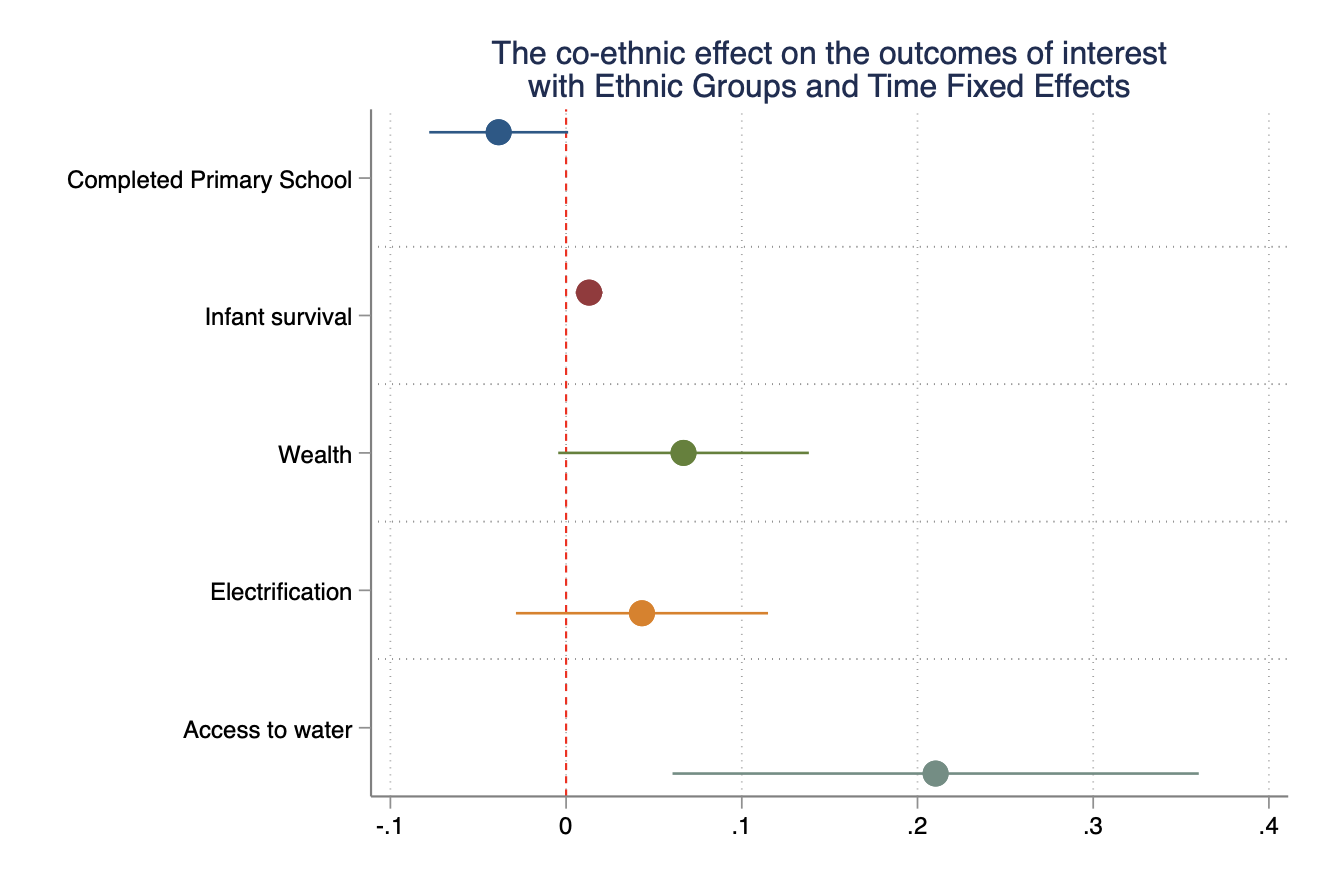
\includegraphics[width=.9\linewidth]{coeth_ethFE.png}
\caption{Effect of co-ethnicity on outcomes of interest with ethnic group and time fixed effects.}
\label{fig:coeet}
\note{In this figure, I present the estimates of the co-ethnicity variable on primary school completion, infant survival, wealth, electrification and access to clean drinking water. The bands represent the 90\% confidence interval and the standard errors are clustered on ethnic groups. All estimates include ethnic group, time and age fixed effects.}
\end{figure}

\begin{table}[!h]

\caption{Ethnic favoritism and democracy results. \label{tab:ethdem}}
\centering
\resizebox{\linewidth}{!}{
\begin{threeparttable}
\begin{tabular}[t]{lccccc}
\toprule
  & \specialcell{(1) \\ Schooling} & \specialcell{(2) \\ Infant Survival} & \specialcell{(3) \\ Wealth} & \specialcell{(4) \\ Electrification} & \specialcell{(5) \\ Clean Water}\\
\midrule
$Democracy\times Coethnic$ & \num{0.033} & \num{-0.004} & \num{-0.024} & \num{0.154}*** & \num{0.279}*\\
 & (\num{0.051}) & (\num{0.008}) & (\num{0.064}) & (\num{0.043}) & (\num{0.142})\\
$Anocracy\times Coethnic$ & \num{0.030}** & \num{0.001} & \num{-0.085} & \num{0.067}* & \num{0.297}*\\
 & (\num{0.014}) & (\num{0.005}) & (\num{0.053}) & (\num{0.039}) & (\num{0.162})\\
\midrule
Mean & \num{0.649} & \num{0.905} & \num{0.275} & \num{0.351} & \num{0.216}\\
N & \num{1146305} & \num{2516753} & \num{756737} & \num{822353} & \num{822353}\\
\bottomrule
\multicolumn{6}{l}{\rule{0pt}{1em}* p $<$ 0.1, ** p $<$ 0.05, *** p $<$ 0.01}\\
\end{tabular}
\begin{tablenotes}
\item[1] \footnotesize{In this table, I am reporting the estimates of equation \ref{eq2}. 
                      I present the results of the interaction between the coethnic variable 
                      and \textit{Polity IV } groups on primary school completions in column 1, 
                      infant survival in column 2, wealth quintile in column 3, electrification in 
                      column 4 and access to clean drinking water in column 4. Primary school completion 
                      is a dummy variable that is equal to one if a person completed primary school and 
                      zero otherwise. Infant survival is a dummy variable that is equal to one if an infant 
                      survived the first 12 months of life. Electrification is a dummy variable that is equal 
                      to one if a household has electricity. Finally, access to clean drinking water is an 
                      ordinal variable that has values from 1, worst water source, to 4.}
\item[2] Democracies have a \textit{Polity IV } $\in [10, 5]$, anocracies have a \textit{Polity IV } 
                      $\in [4, -5]$ and autocracies, the omitted group, have a \textit{Polity IV } $<-5$.
\item[3] \footnotesize{Standard errors are clustered on country specific ethnic groups. All 
                      results include ethnic group, time and age fixed effects.}
\end{tablenotes}
\end{threeparttable}}
\end{table}



\begin{figure}[!htb]
\centering
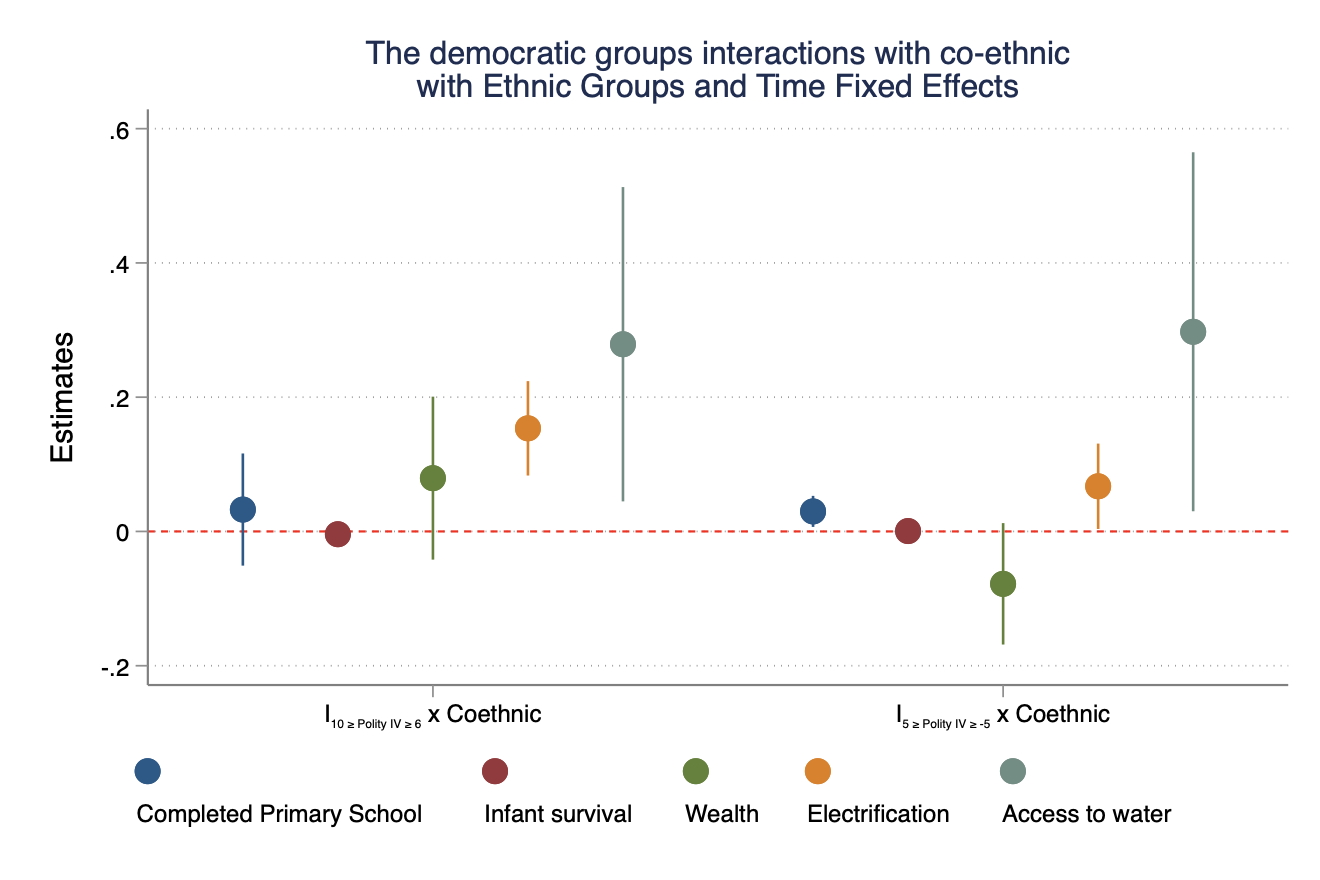
\includegraphics[width=.9\linewidth]{coeth_dem_ethFE.png}
\caption{With ethnic groups and time fixed  effects.}
\label{fig:coedemet}
\note{In this figure, I present the effect of the interaction between co-ethnicity variable and Polity groups on primary school completion, infant survival, wealth, electrification and access to clean drinking water. Democracies have a \textit{Polity IV } $\in [10, 5]$, anocracies have a \textit{Polity IV } $\in [4, -5]$ and autocracies, the omitted group, have a \textit{Polity IV } $<-5$. The bands represent the 90\% confidence interval and the standard errors are clustered on ethnic groups. All estimates include ethnic group, time and age fixed effects.}
\end{figure}


\begin{figure}[!htb]
\centering
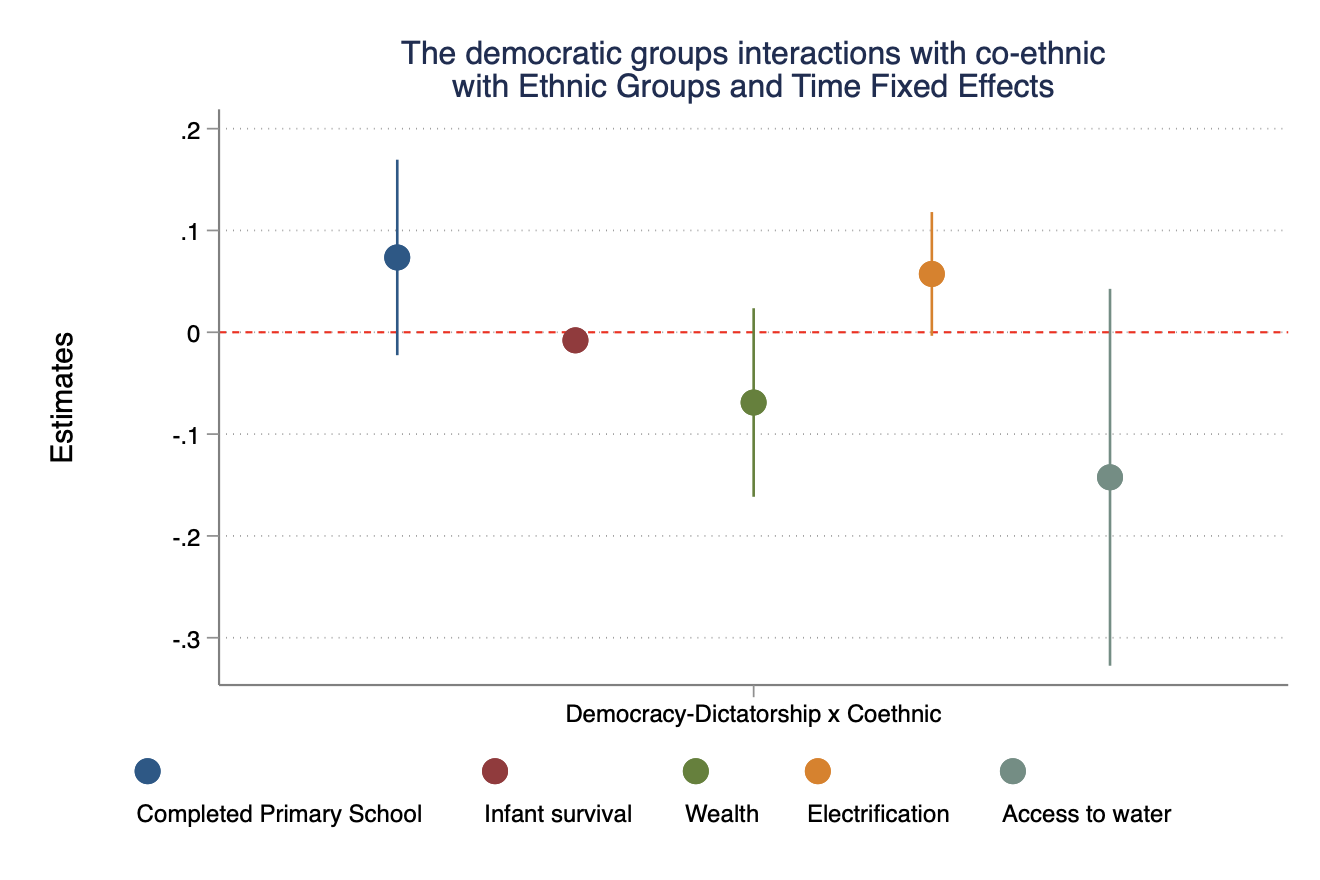
\includegraphics[width=.9\linewidth]{coeth_demdic_ctFE.png}
\caption{Effect of the interaction between co-ethnicity and Democracy-Dictatorship Index on outcomes of interest with ethnic groups and time fixed effects.}
\label{fig:demdicindex}
\note{In this figure, I present the effect of the interaction between co-ethnicity variable and the Democracy-Dictatorship on primary school completion, infant survival, wealth, electrification and access to clean drinking water. In this specification, I used the Democracy-Dictatorship index as a measure of democracy. The Democracy-Dictatorship index is an indicator variable that is equal to 1 if a country is democratic and zero otherwise. The bands represent the 90\% confidence interval and the standard errors are clustered on ethnic groups. All estimates include ethnic group, time and age fixed effects.}
\end{figure}



\begin{table}[!h]

\caption{Ethnic favoritism and continuous democracy measure results. \label{tab:ethdemcont}}
\centering
\resizebox{\linewidth}{!}{
\begin{threeparttable}
\begin{tabular}[t]{lccccc}
\toprule
  & \specialcell{(1) \\ Schooling} & \specialcell{(2) \\ Infant Survival} & \specialcell{(3) \\ Wealth} & \specialcell{(4) \\ Electrification} & \specialcell{(5) \\ Clean Water}\\
\midrule
$PolityIV\times Coethnic$ & \num{0.01}* & \num{0.00} & \num{0.00} & \num{0.01}*** & \num{0.02}*\\
 & (\num{0.00}) & (\num{0.00}) & (\num{0.01}) & (\num{0.00}) & (\num{0.01})\\
\midrule
N & \num{1135494} & \num{2511731} & \num{750704} & \num{816320} & \num{816320}\\
Mean & \num{0.65} & \num{0.91} & \num{0.27} & \num{0.35} & \num{0.22}\\
Birth Year FE & X & X & X & X & X\\
Age FE & X & X & X & X & X\\
Country Specific Ethnic Group FE & X & X & X & X & X\\
\bottomrule
\multicolumn{6}{l}{\rule{0pt}{1em}* p $<$ 0.1, ** p $<$ 0.05, *** p $<$ 0.01}\\
\end{tabular}
\begin{tablenotes}
\item[1] \footnotesize{In this table, I am reporting the estimates of equation \ref{eq1}. 
                      I present the results of the interaction between the coethnic variable and 
                      \textit{Polity IV } groups on primary school completions in column 1, infant 
                      survival in column 2, wealth quintile in column 3, electrification in column 4 
                      and access to clean drinking water in column 4. Primary school completion is a 
                      dummy variable that is equal to one if a person completed primary school and 
                      zero otherwise. Infant survival is a dummy variable that is equal to one if an 
                      infant survived the first 12 months of life. Electrification is a dummy variable
                      that is equal to one if a household has electricity. Finally, access to clean 
                      drinking water is an ordinal variable that has values from 1, worst water source, to 4.}
\item[2] \footnotesize{\textit{Polity IV } score in this specification is continuous. It takes
                      values that range from most autocratic $-10$ to most democratic $10$}
\item[3] \footnotesize{Standard errors are clustered on ethnic groups. All 
                      results include ethnic group, time and age fixed effects.}
\end{tablenotes}
\end{threeparttable}}
\end{table}


\begin{table}[!h]

\caption{Ethnic favoritism and continuous democracy measure results. \label{tab:ethdemdic}}
\centering
\resizebox{\linewidth}{!}{
\begin{threeparttable}
\begin{tabular}[t]{lccccc}
\toprule
  & \specialcell{(1) \\ Schooling} & \specialcell{(2) \\ Infant Survival} & \specialcell{(3) \\ Wealth} & \specialcell{(4) \\ Electrification} & \specialcell{(5) \\ Clean Water}\\
\midrule
$D-DIndex\times Coethnic$ & \num{0.073} & \num{-0.008} & \num{0.111} & \num{0.057} & \num{-0.142}\\
 & (\num{0.058}) & (\num{0.007}) & (\num{0.074}) & (\num{0.037}) & (\num{0.112})\\
\midrule
Mean & \num{0.649} & \num{0.905} & \num{0.275} & \num{0.351} & \num{0.216}\\
N & \num{988262} & \num{2070052} & \num{452222} & \num{453673} & \num{453673}\\
\bottomrule
\multicolumn{6}{l}{\rule{0pt}{1em}* p $<$ 0.1, ** p $<$ 0.05, *** p $<$ 0.01}\\
\end{tabular}
\begin{tablenotes}
\item[1] \footnotesize{In this table, I am reporting the estimates of equation \ref{eq1}. 
                      I present the results of the interaction between the coethnic variable and 
                      \textit{Polity IV } groups on primary school completions in column 1, infant 
                      survival in column 2, wealth quintile in column 3, electrification in column 4 
                      and access to clean drinking water in column 4. Primary school completion is a 
                      dummy variable that is equal to one if a person completed primary school and 
                      zero otherwise. Infant survival is a dummy variable that is equal to one if an 
                      infant survived the first 12 months of life. Electrification is a dummy variable
                      that is equal to one if a household has electricity. Finally, access to clean 
                      drinking water is an ordinal variable that has values from 1, worst water source, to 4.}
\item[2] \footnotesize{\textit{Polity IV } score in this specification is continuous. It takes
                      values that range from most autocratic $-10$ to most democratic $10$}
\item[3] \footnotesize{Standard errors are clustered on ethnic groups. All 
                      results include ethnic group, time and age fixed effects.}
\end{tablenotes}
\end{threeparttable}}
\end{table}



\begin{center}
\begin{table}[H]
\centering
\caption{Institutions' effects on ethnic \\ favoritism: using light data.}
\label{tab:hodler}
\begin{tabular}{lcccccccc}
\hline 
 & \multicolumn{3}{c}{Ethnologue} &  &  & \multicolumn{3}{c}{GREG}\tabularnewline
\cline{2-4} \cline{7-9} 
 &  & $Light_{ict}$ &  &  &  &  & $Light_{ict}$ & \tabularnewline
\hline 
\textbf{Panel A: Ethnic Favoritism} &  &  &  &  &  &  &  & \tabularnewline
$Coethnic_{ict}$ &  & 0.061 &  &  &  &  & 0.097{**} & \tabularnewline
 &  & (0.051) &  &  &  &  & (0.036) & \tabularnewline
\textbf{Panel B: Ethnic favoritism} &  &  &  &  &  &  &  & \tabularnewline
\textbf{and institutions} &  &  &  &  &  &  &  & \tabularnewline
$Coethnic_{ict}\times Polity_{ct}$ &  & -0.076 &  &  &  &  & -0.041 & \tabularnewline
 &  & (0.204) &  &  &  &  & (0.131) & \tabularnewline
%$Coethnic_{ict}\times Anocracy_{ct}$ &  & 0.192{*} &  &  &  &  & 0.027 & \tabularnewline
% &  & (0.090) &  &  &  &  & (0.773) & \tabularnewline
\hline 
\end{tabular}
\end{table}
\end{center}

\pagebreak
\bibliography{ethnicfav}
\pagebreak
\nocite{*}

\begin{appendices}


%\begin{table}[!htbp]
%\caption{Effect of ethnic favoritism on variables of interest by Polity IV group.} \label{tab:ethgrps}
% \estwide{ethnic_fav_grps.tex}{10}{lccccc}
%\end{table}

\section{Data Appendix}

\begin{table}[!htb]
\caption{The number of co-ethnic and non-coethnic observations in each polity score.}
\label{tab5}
\resizebox{\textwidth}{!}{%
\begin{tabular}{l|ll}
Polity Score & \begin{tabular}[c]{@{}l@{}}Not a \\ Co-ethnic Leader\end{tabular} & Co-ethnic Leader \\ \hline
-9           & 130,381                                                          & 26,648          \\
-8           & 27,207                                                           & 1,613           \\
-7           & 241,663                                                          & 37,388          \\
-6           & 37,936                                                           & 3,701           \\
-5           & 17,965                                                           & 5,928           \\
-4           & 23,396                                                           & 1,564           \\
-3           & 12,863                                                           & 3,147           \\
-2           & 9,870                                                            & 1,338           \\
-1           & 44,950                                                           & 19,604          \\
0            & 16,269                                                           & 1,336           \\
1            & 6,624                                                            & 340             \\
2            & 6,345                                                            & 200             \\
3            & 7,604                                                            & 273             \\
4            & 31,825                                                           & 1,689           \\
5            & 4,550                                                            & 539             \\
6            & 13,091                                                           & 3,329           \\
7            & 18,290                                                           & 4,054           \\
8            & 5,890                                                            & 1,674           \\
9            & 37                                                               & 1,762          
\end{tabular}%
}
\end{table}

\newpage
\begin{table}[!htb]
\caption{The number of co-ethnic and non-coethnic observations in polity groups.}
\label{tab6}
\resizebox{\textwidth}{!}{%
\begin{tabular}{l|ll}
Polity Score       & \begin{tabular}[c]{@{}l@{}}Not a \\ Co-ethnic Leader\end{tabular} & Co-ethnic Leader \\ \hline
Democracy          & 37,308                                                           & 10,819          \\
Open Anocracy      & 56,948                                                           & 3,041           \\
Closed Anocracy    & 125,313                                                          & 32,917          \\
Autocracy          & 437,187                                                          & 69,350          \\
Failed or Occupied & 1,229                                                            & 92             
\end{tabular}%
}
\end{table}

\subsection{Countries included in the data-set}
I used data from twenty-one countries. These countries and the distribution of observations are presented in table \ref{countries}.

\begin{table}[!htb]
\centering
\caption{Number of Observations by country.}
\label{countries}
\resizebox{\textwidth}{!}{%
\begin{tabular}{@{}lll@{}}
\toprule
Country                   & Number of observations & Percent \\ \midrule
Angola                    & 12,145                 & 1.57    \\
Cameroon                  & 31,777                 & 4.10    \\
Congo Democratic Republic & 28,224                 & 3.65    \\
Benin                     & 41,969                 & 5.42    \\
Ethiopia                  & 29,437                 & 3.80    \\
Ghana                     & 27,571                 & 3.56    \\
Guinea                    & 22,107                 & 2.86    \\
Cote d'Ivoire             & 18,403                 & 2.38    \\
Kenya                     & 58,278                 & 7.53    \\
Malawi                    & 68,081                 & 8.79    \\
Mali                      & 42,372                 & 5.47    \\
Mozambique                & 18,179                 & 2.35    \\
Namibia                   & 2,872                  & 0.37    \\
Niger                     & 29,963                 & 3.87    \\
Nigeria                   & 90,445                 & 11.68   \\
Senegal                   & 92,990                 & 12.01   \\
South Africa              & 20,249                 & 2.62    \\
Zimbabwe                  & 16,987                 & 2.19    \\
Uganda                    & 47,739                 & 6.17    \\
Burkina Faso              & 36,834                 & 4.76    \\
Zambia                    & 37,582                 & 4.85    \\ \hline
Total                     & 774,204                & 100     \\ \bottomrule
\end{tabular}%
}
\end{table} 
\end{appendices}
\end{document}
